\documentclass[twoside,11pt]{article}

\usepackage{jmlr2e}
\usepackage{amsmath}
\usepackage[]{algorithm2e}


\ShortHeadings{Optimal spike-based signal representation on a neuromorphic chip}{Optimal spike-based signal representation on a neuromorphic chip}
\firstpageno{1}

\begin{document}


\title{Optimal spike-based signal representation\\on a neuromorphic chip}

\author{\name Julian B\"uchel \email jubueche@ethz.ch \\
       \addr Institute of Neuroinformatics\\
       University of Z\"urich, ETH Z\"urich \\
       Z\"urich, ZH, Switzerland}

\editor{}

\maketitle

\tableofcontents
\newpage

\begin{abstract}%   <- trailing '%' for backward compatibility of .sty file
The question of how a population of neurons encodes a signal in the brain is one of the
most fundamental, yet unsolved problems in neuroscience. In general, it is believed that
neurons encode information via their firing rate, specifically via Poisson rate codes (\cite{Maass:2002:RCW:639717.639718}).
Due to the unreliability induced by the Poisson-process, the representation error using Poisson
rate codes only scales with $\frac{1}{\sqrt{M}}$, where $M$ is the number of spikes.
This leads to the fact that many spikes fired are redundant and are thus a waste of energy,
contrary to the fact that neural agents seek to minimize energy consumption. This
leads to the natural question of whether there exists a more complex system that
represents signals with a representation error that scales with $\frac{1}{M}$, making better
use of individual spikes.
  

\end{abstract}

\begin{keywords}
  Neuromorphic Processors, Optimal Signal Representation, Neural Coding
\end{keywords}

\section{Introduction}

Recently, \cite{wiel2017learning} proposed a local online learning rule, guiding a recurrently connected
network into a tightly balanced domain. The authors showed that keeping a tight balance,
commonly referred to as E/I-balance, improves the representation error, leads to sparser spike
trains, and assigns higher value to individual spikes.
The goal of this thesis is to implement this local learning rule on a neuromorphic chip in-the-loop,
meaning that weights are iteratively loaded onto the neuromorphic chip and updated offline using
responses obtained from the chip. Furthermore, this thesis aims at investigating the
possibility of implementing this learning rule directly on-chip using mixed analog/digital
circuits, by identifying possible weaknesses of the proposed theory and resolving them.
Having a circuit that learns optimal spike-based signal representation is desirable from many points of view.
From a neuroscience perspective, the emulation of such learning rule in a biologically realisitic setting
would show that brains are indeed capable of implementing a more complex way of representing signals
and might lead to new theories on how this is actually achieved in a pure biological setting.
Additionally, the possibility of representing signals with high precision while saving a lot of
energy might be applicable in neural agents, operating autonomously in environments that are providing
continous stimuli or IoT devices requiring ultra low power consumption.
In a more classical Machine Learning setting, learning such a network would
correspond to a standard Autoencoder (\cite{Vincent:2008:ECR:1390156.1390294}) with a high dimensional, sparse latent space, possibly
opening up new ways of performing learning tasks in neural agents.


\section{Theory: Representing signals spike-by-spike}

\subsection{Network dynamics}
%Define voltage equation(diff and explicit), rate equation, reconstructed x
%State assumptions such as fully connected, not respecting Dales law. Also state that these
%assumptions can be relaxed and reference to paper that achieves this

[\cite{wiel2017learning}] In this work, we assume that we have a population of $N$ neurons into which $N_x$ continous
signals are fed using a linear transformation $\mathbf{F}$. We furthermore assume that the population
of $N$ neurons is fully interconnected by a matrix $\mathbf{\Omega}$. It is thus beneficial to assume 
the computationally efficient Leaky Integrate-and-Fire (LIF) neuron model (\cite{Lapicque}). 
The network dynamics can thus be written as

\begin{equation} \label{voltage_dynamic_diff}
    \dot{V}(t) = -\lambda V(t) + \mathbf{F^T}c(t) + \mathbf{\Omega} o(t) 
\end{equation}

Where $c(t)$ is the input signal at time $t$ and $o(t)$ the spike train of the population, also at
time $t$. By defining a filtered version of the input $c$ and the spike train $o$, we can integrate Equation \ref{voltage_dynamic_diff}
to
%! Not V(t+1)?!
\begin{equation} \label{voltage_dynamic_explicit}
    V(t) = \mathbf{F^T}x(t) + \mathbf{\Omega} r(t)
\end{equation}
where we define
\begin{equation} \label{rate_diff}
    \dot{r}(t) = -\lambda r(t) + o(t)
\end{equation}
and 
\begin{equation} \label{input_diff}
    \dot{x}(t) = -\lambda x(t) + c(t)
\end{equation}
For the simulations conducted in this thesis, uncorrelated inputs where used. These were generated
by simply convolving white noise with a gaussian filter of width $\sigma$. An example of a typical
input used throughout this thesis is presented in Figure \ref{fig:input}.

\begin{figure}[!htb]
    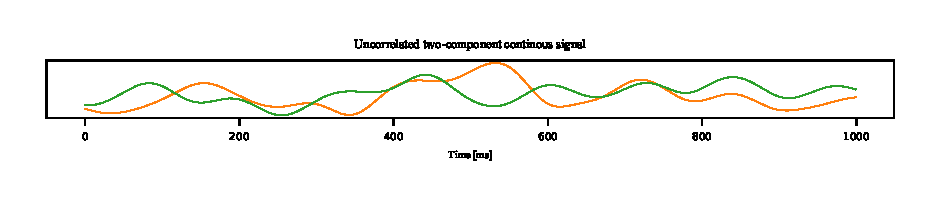
\includegraphics[width = \columnwidth, height=3cm]{figures/input.eps}
    \caption{Input $x$ of dimension $N_x = 2$ shown over a period of 1000 ms.}
    \label{fig:input}
\end{figure}

It should be noted that for the sake of mathematical simplicity, as well as ease of
transformation to a neuromorphic chip, this setup does not respect Dales law (\cite{Dale1935}), as it
allows for neurons to be excitatory and inhibitory at the same time. However, (\cite{wiel2017learning})
also derives learning rules that respect the more biologically plausible setup.

We furthermore assume a readout layer, or decoder, that reconstructs the input $x$ using
the rates exposed by the population. The reconstructed signal can be defined as

\begin{equation*}
    \mathbf{\hat{x}} = \mathbf{Dr}
\end{equation*} 
where the decoder $\mathbf{D}$ is a matrix of size ($N_x$,$N$), $\mathbf{r}$ is a matrix of shape
($N$,$N_\textnormal{time}$) and $\mathbf{x}$ is a matrix of shape ($N_x$,$N_\textnormal{time}$).

\subsection{The optimal decoder}

Keeping in mind the goals that we are following, namely low reconstruction error, low firing
rates and even distribution across neurons, we can define the following loss function, balancing
low reconstruction error with sparse (\textit{l1}-cost) and dense (\textit{l2}-cost) spike trains.

\begin{equation} \label{loss_function_optimal_decoder}
    L^* = \min_{o} \|\mathbf{x} - \mathbf{Dr}\| ^2_2 + \mu \|\mathbf{r}\|_2^2 + \nu \|\mathbf{r}\|_1
\end{equation}

Because of Equation \ref{rate_diff}, one can see that enforcing \textit{l2}-sparsity allows for
dense population codes (since it keeps the rates genereally low, but does not enforce 0 values). 
In contrast, \textit{l1}-sparsity encourages 0 values in the rates, which correponds to sparse spike trains (\cite{Tibshirani1996}).
This loss function gives us an explicit formula for the optimal decoder that is achievable by the network.
By taking the derivative of Equation \ref{loss_function_optimal_decoder} with respect to $\mathbf{D}$ and setting it to \textbf{0}, we get

\begin{equation*}
    \mathbf{D}^* = \mathbf{xr^T}(\mathbf{rr^T})^{-1}
\end{equation*}


\subsection{Optimal network connectivity}

Following \cite{wiel2017learning}, we will now discuss how to optimize the network topology.
In particular the synaptic weights and the thresholds
under the assumption that the decoder is fixed. Note that letters such as
$r$ are not bold and thus stand for a vector in time, $r(t)$, which is abbreviated for clarity.
The main idea (\cite{Bourdoukan:2012:LOS:2999325.2999390}) behind the
following derivation is that a neuron in the population should only spike if it
contributes to the reduction of the loss function.
This means that

\begin{equation} \label{loss_smaller}
  \textit{L(neuron n spikes)} < \textit{L(neuron n does not spike)}
\end{equation}

Using Equation \ref{loss_function_optimal_decoder}, $\textit{L(neuron n spikes)}$ can be
written as

\begin{equation*}
  \textit{L(neuron n spikes)}=\|c-Dr-D_n \|_2^2+\mu\|r+e_n\|^2_2+\nu\|r+e_n\|_1
\end{equation*}
where $e_n$ is the unit vector with $(e_n)_j = 1$ if $j=n$ and 0 else.

We observe that
\begin{equation} \label{rate_plus_unit_l2}
  \|r+e_n\|^2_2 = (\sum_{i,i \neq n}r_i) + (r_n+1)^2 = \|r\|^2_2 + 2r_n + 1
\end{equation}
and
\begin{equation} \label{rate_plus_unit_l1}
  \nu \|r + e_n\|_1 = \nu (\sum_{i,i\neq n}|r_i|) + \nu |r_n+1| =^* \nu (\sum_{i,i\neq n}|r_i|) + \nu |r_n| +\nu = \nu \|r\|_1 + \nu  
\end{equation}
where * holds because $\forall t \; r(t) \geq 0$.
Using Equations \ref{rate_plus_unit_l2} and \ref{rate_plus_unit_l1} we can rewrite Equation
\ref{loss_smaller} to

\begin{equation} \label{network_dynamics}
  D_n^Tc - D_n^TDr - \mu r_n > \frac{1}{2} (\| D_n\|^2_2 + \mu + \nu) 
\end{equation}

This condition enforces that neuron $n$ only fires a spike, when it contributes
to the reduction of the global error. We observe,
under the assumption that the decoder is fixed, that the r.h.s. is constant and the l.h.s. is 
time-dependent, as it depends on $c$ and $r$.
It is therefore natural to denote the voltage of neuron $n$ as

\begin{equation} \label{voltage_via_dynamics}
  V_n(t) = D_n^Tc(t) - D_n^TDr(t) - \mu r_n 
\end{equation}
and the threshold of the $n$-th neuron as
\begin{equation} \label{threshold_via_dynamics}
  T_n = \frac{1}{2} (\| D_n\|^2_2 + \mu + \nu)
\end{equation}

using the differential equations \ref{input_diff} and \ref{rate_diff}, as well as Equation \ref{voltage_dynamic_diff}
we rewrite Equation \ref{voltage_via_dynamics} to

\begin{equation*}
  V(t) = \mathbf{F^T}x(t) + \mathbf{\Omega} o(t)
\end{equation*}
where we substituted $\mathbf{F} = \mathbf{D}$ and $\mathbf{\Omega} = -\mathbf{D^TD} - \mu \mathbf{I} = -\mathbf{F^TF} - \mu \mathbf{I}$, which are the optimal feed-forward and
recurrent weights in the network, with respect to the decoder.

We also note that since $\mathbf{\Omega} = -\mathbf{D^TD} - \mu \mathbf{I}$, we have $T = \frac{1}{2}(\textnormal{diag}(\mathbf{\Omega}) + \nu)$.
This way the error dictates the produced spike train, hence \emph{error-driven coding}.

Since neurons have a "fixed" threshold, Equation \ref{threshold_via_dynamics} can be seen
as a constraint on the decoder length for a neuron by simply rewriting it to

\begin{equation*}
  \|D_n\|_2^2 = 2T_n - \mu - \nu
\end{equation*} 


\subsection{Learning optimal recurrent connectivity}

We have seen from the previous section that the voltage encodes the global loss and
that a neuron fires a spike only to reduce the reconstruction error.
This corresponds to the hypothesis that a tightly balanced network exhibits a low reconstruction
error.
This however corresponds to the state where $\mathbf{x} - \mathbf{\hat{x}} \approx 0$.
We observe that the neuron has only access to the linearly transformed version: $F_n^T\mathbf{x} - F_n^TD\mathbf{r}$. 
However, this value should also be close to zero, as it reflects part of the reconstruction error.

\begin{equation} \label{balanced_voltage}
  \begin{split}
    \epsilon_n &= F^T_n\mathbf{x}-F^T_n\mathbf{\hat{x}} \\
    &= F_n^T - F^T_n\mathbf{Dr} \\
    &\approx 0
  \end{split}
\end{equation}

We furthermore observe, using the optimal feed-forward and recurrent connections, that Equation
\ref{balanced_voltage} corresponds to the network dynamics obtained in Equation \ref{voltage_dynamic_explicit}.
We can conclude that the signal is represented optimally if $\Omega_n = -F^T_n\mathbf{D}$, $\epsilon_n = V_n \approx 0$ and
$\mathbf{D} = \mathbf{D}^*$.
From this, we are now able to derive a learning rule for the recurrent weights, that will yield
the optimal solution.

In order to achieve a balanced network, it is desirable that over the long run, the
membrane voltages before and after a presynaptic spike cancel each other:

\begin{equation} \label{loss_voltage_before_after}
  L(t_j) = \| \frac{1}{2} (V^{\textnormal{before}}(t_j)+V^{\textnormal{after}}(t_j)) \| ^2_2
\end{equation}
Note that we add the two voltages since we assume that the voltage jumps from the positive to the
negative domain.
After the arrival of a presynaptic spike at time $t_j$ of neuron with index $k(j)$, the voltages are changed and the following relation is formed:

\begin{equation} \label{relation_voltage_before_after}
  V^{\textnormal{after}} = V^{\textnormal{before}} + \mathbf{\Omega} e_{k(j)}
\end{equation}

where $e_{k(j)}$ is the unit vector with 1 at the position of the neuron that spiked.
Using this relation we can rewrite the Equation \ref{relation_voltage_before_after} to

\begin{equation*} 
  L = \|V^{\textnormal{before}} + \frac{1}{2}\mathbf{\Omega} e_{k(j)}\|^2_2
\end{equation*}

this term has the derivative, with respect to $\Omega_{n,k}$:

\begin{equation*}
    \Delta \Omega_{n,k} = -2V^{\textnormal{before}}_n - \Omega_{n,k}
\end{equation*}

if neuron $k$ spiked. The connection $\Omega_{n,k}$ is the connection from the spiking, presynaptic neuron with index $k$ to the $n$-th neuron.

If we induce a small \textit{l2}-cost on the rates, $\mathbf{\Omega}$ should ideally converge towards $-\mathbf{F^TD} - \mu \mathbf{I}$. This causes a minor change in the learning rule for the recurrent weights:
\begin{equation*}
    \Delta \Omega_{n,k} = -2(V^{\textnormal{before}}_n + \mu r_n) - \Omega_{n,k} - \mu \delta_{n,k}
\end{equation*}

where $\delta_{n,k}$ is $[e_n]_j$ and therefore 1 if $n =j$.


\subsection{Simulation and results}
%State the pseudo code when using only recurrent connections.
%Show figures of the weight convergence, the error convergence, variance of membrane potential
%mean firing rate and actual decoding that is happening.
Learning the feed-forward connections happens on a much slower timescale and thus requires
far more training iterations. Since the DYNAP-SE operates on a much slower, biologically
more plausible timescale (\cite{DBLP:journals/corr/abs-1708-04198}), training takes orders of magnitude longer. We therefore decided to omit
learning the feed-forward weights and keep them constant after an initial random initialisation.
The pseudo code presented below was adapted from (\cite{wiel2017learning}) and shows the learning procedure.

\vspace{1cm}
\IncMargin{1em}
\begin{algorithm}[H]
  \DontPrintSemicolon
  \label{algorithm_simulation}
  \KwIn{Number of training iterations $N_\textnormal{iter}$}
  \KwOut{Learned recurrent matrix $\mathbf{\Omega}$}
  \BlankLine
  $T \leftarrow \textnormal{N}_\textnormal{iter} \cdot \textnormal{N}_{\textnormal{time}}$\;
  $\textit{thresh} \leftarrow 0.5$ \;
  \For{$i \leftarrow 0$ \KwTo $T$}{
    \If(\tcp*[h]{Generate new input}){$i \; \textnormal{mod} \; \textnormal{N}_{\textnormal{time}} = 0$}{
      $Input \leftarrow \mathcal{N}(\mathbf{0}, \mathbf{I})$ \;
      $Input \leftarrow A \cdot (Input \ast w)$ \;
    } 
    $t \leftarrow (i \; \textnormal{mod} \; \textnormal{N}_{\textnormal{time}})+1$ \;
    $V_t \leftarrow (1-\lambda dt) \cdot V_{t-1}+dt \cdot \mathbf{F^T}\textnormal{Input}_t+\mathbf{\Omega} o_{t-1}+\epsilon \cdot \mathcal{N}(0,1) $ \;
    $x_t \leftarrow (1-\lambda dt)\cdot x_{t-1}+dt\cdot  \textnormal{Input}_t$ \;

    $(\textnormal{max},k) \leftarrow \textnormal{arg max}(V_t - \textit{thresh}-0.01 \cdot \mathcal{N}(0,1))$ \;
    \eIf(\tcp*[h]{Neuron k spiked}){$\textnormal{max} \geq 0$}{
      $\Omega_k \leftarrow \Omega_k-\epsilon_\Omega \cdot (\beta \cdot (V_t + \mu \cdot r_{t-1})+\Omega_k+\mu \cdot I_k)$ \;
      $r_t \leftarrow r_{t-1} + I_k$ \;
    }
    {
      $r_t \leftarrow r_{t-1}$
    }
    $r_t \leftarrow (1 - \lambda dt) \cdot r_t$ \;
  }
  \caption{Algorithm describing the learning procedure without learning the feed-forward weights.
  $\Omega_k$ and $I_k$ reference the
  $k$-th column of the respective matrix and $\ast$ is the convolution operator.}
\end{algorithm}
\DecMargin{1em}
\vspace{1cm}

Given the randomly initialized feed-forward matrix $\mathbf{F}$, we can measure the distance
between $\mathbf{\Omega}$ and $\mathbf{\Omega}^* = \mathbf{-F^TF}$, even if $\mathbf{F}$ is not learned.
As expected, the recurrent connection matrix converges towards the
optimal connectivity (Figure \ref{fig:convergence}(i)).
Initially, the network is in an unbalanced state and the
voltage predominantly reflects the transformed input.
After learning the recurrent weights, incoming excitatory signals are matched by
recurrent inhibition to keep the network in a tightly balanced state. This effect can be
observed in Figure \ref{fig:convergence}(iv) where we show the variance of the
membrane potential over time. By converging towards the optimal recurrent connection
and keeping the network in a tight balance, we fulfill the conditions necessary
for representing the signal optimally. The result of this can be seen
in Figure \ref{fig:convergence}(iii), where
the reconstruction error converges towards the discretization limit imposed by the
neurons. Since the learning rule keeps the network in a tight balance, no spike is fired
unnecessarily. Each spike, following Equation \ref{loss_smaller}, contributes
to reducing the global reconstruction error. This way, the resulting spike train sparsifies,
which can be observed in Figure \ref{fig:convergence}(ii). \\

\begin{figure}[!htb]
  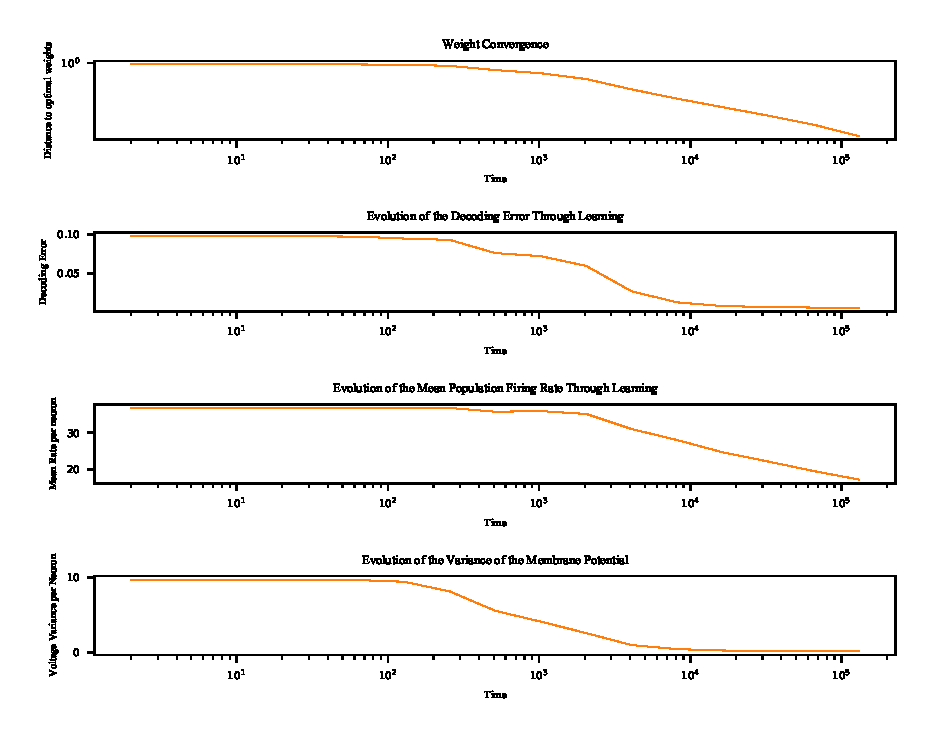
\includegraphics[width = \columnwidth, height=12cm]{figures/convergence.eps}
  %! Correct caption please
  \caption{(i) Convergence of optimal weights
  (ii) Convergence of error (iii) Convergence of mean firing rate (iv) Convergence
  of voltage variance}
  \label{fig:convergence}
\end{figure}
\newpage

To see the effect of learning, we trained the network for 140
iterations on different signals from the same domain. After the training process, we
computed the optimal decoder for the network using $\mathbf{\Omega}_{\textnormal{initial}}$ and
for the network using $\mathbf{\Omega}_{\textnormal{post learning}}$. We then generated a
new input $x$, which was then fed into the networks.
Using the decoder previously computed, we then reconstructed the signal and
compared the reconstruction quality. Figure \ref{fig:reconstruction} shows the different
reconstructions and spike trains of each network. As expected, results using
$\mathbf{\Omega}_{\textnormal{initial}}$ produced a poor reconstruction
compared to the network using $\mathbf{\Omega}_{\textnormal{post learning}}$.
It is also visible from the spike trains that the voltage initially
only represents the transformed input and later becomes more distributed across
the population.


\begin{figure}[!htb]
  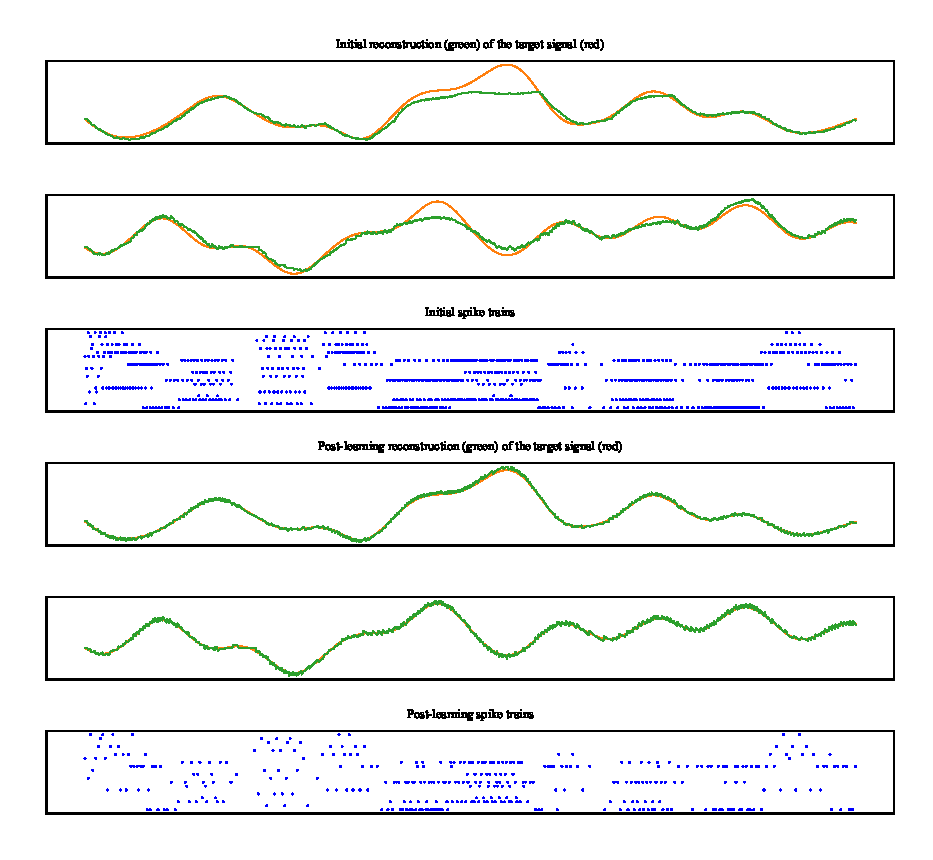
\includegraphics[width = \columnwidth, height=14cm]{figures/reconstruction.eps}
  \caption{The two-dimensional input is reconstructed pre-learning (row 1 \& 2) and
  post-learning (row 4 \& 5). Due to the evolving tight balance, the population
  spike trains sparsify (row 3 \& 6).}
  \label{fig:reconstruction}
\end{figure}
\newpage

\subsection{Limitations of the theory} \label{sec:limitations}
%Discrete weights, taking the neuron with the maximum voltage above threshold to compute
%the rate vectors and do the updates. (Need to check if fails when using all neuons)
%Provide figures showing: Number of bins vs. recon error after 14000 iterations.
%Another figure showing two figures when using all neurons in the update.
Unfortunately, the theory proposed by (cite Brendel) has some limitations: \\
1) Discretization of the weights causes unsuccessful learning of the recurrent matrix and therefore
does not lead to improved sparsity and reconstruction error. \\
2) Updating the rate, as well as all outgoing connections of \emph{all} neurons that spiked,
results in no improvement of the mean firing rate and the reconstruction error.
Furthermore, the update utilizes the voltage \emph{before} the spike propagated. \\

In this theory, tight balance of the input
currents is of crucial importance. When discretizing the weights, this tight balance can no longer
be achieved and no improvement of the reconstruction error is visible.
Considering that synaptic weights in the human brain actually do have a reasonably high resolution (need citation),
this constraint is solely imposed by the hardware we use and will be resolved in future chip designs
by e.g. using multi-memristive synapses (\cite{Boybat2018}).

\begin{figure}[!htb]
  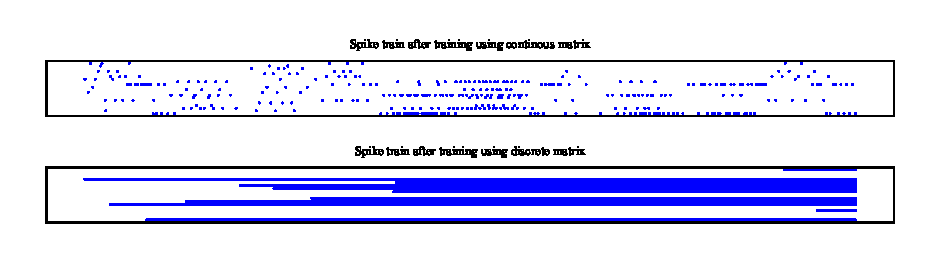
\includegraphics[width = \columnwidth, height=4cm]{figures/spike_train_cont_vs_disc.eps}
  \caption{The spike train after training using continous weights (top), exhibits a usable,
  distributed pattern, while the learned, discretized weight matrix (bottom) shows a subset
  of neurons firing at a high frequency.}
  \label{fig:discrete_spike_trains}
\end{figure}

Assuming a continous timescale, there can not be an instance in time, where two neurons fire simultaneously.
However, in the simulations, as well as on the DYNAP-SE, time is discretized and therefore
the event that two neurons fire at the same time \emph{can} happen.
When adapting Equation \ref{relation_voltage_before_after} to account for this possibility and rewriting
the update rule accordingly, we found that the recurrent weights were still learned. Furthermore, the
variation in the membrane potential also decreased, which is explained by the fact that we are still
minimizing the loss in Equation \ref{loss_voltage_before_after}.
However, the derivation of the optimal network connectivity
in Equation \ref{network_dynamics} falsely assumes only one spike per time.

The only problem that we identified as biologically unrealistic is the fact that the post-synaptic
neuron updates the synaptic weight based on the voltage \emph{before} the spike propagated, meaning
the voltage was not affected by the spike. This problem might be resolved by implementing
a slow changing variable, approximating the voltage before the spike due to the slow update.

\newpage

\begin{figure}[!htb]
  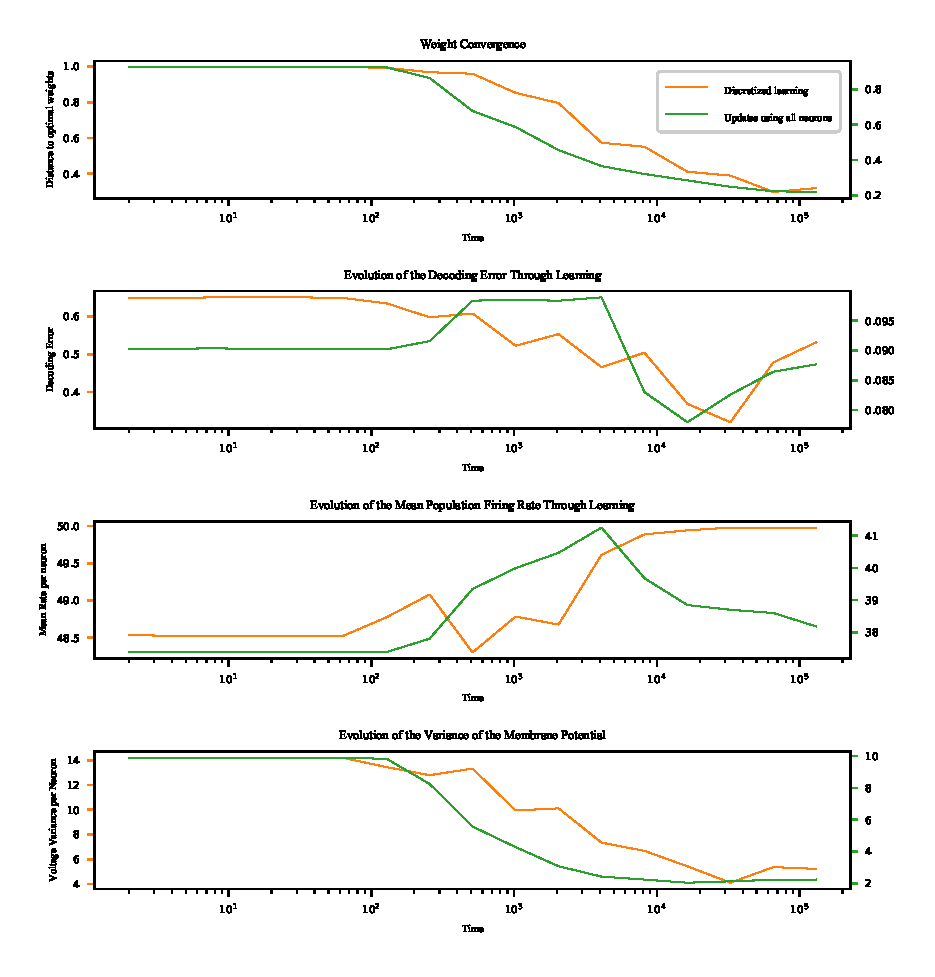
\includegraphics[width = \columnwidth, height=16cm]{figures/convergence_d_vs_ua.eps}
  \caption{Convergence of different properties when learning with discrete weights (orange)
  and performing the updates with respect to all spiking neurons (green).
  It should be noted that the mean firing rate is really high compared to the successful learning (see
  Figure \ref{fig:convergence}).}
  %! Correct caption please
  \label{fig:convergence_ua_discrete}
\end{figure}

\newpage

\section{Hardware: The DYNAP-SE chip} \label{sec:DYNAP-SE}
The DYNAP-SE is a fully custom mixed signal neuromorphic chip developed by Ning Qiao, Saber Moradi,
Fabio Stefanini and Giacomo Indiveri (\cite{DBLP:journals/corr/abs-1708-04198}). It comprises 4 chips, each containing 4 cores with
4x256 neurons following the adaptive exponential integrate-and-fire neuron model (AEI\&F) with a fan-in of 64 and fan-out of 4064.
Each neuron has a Content Adressable Memory (CAM) block, containing 64 addresses representing the pre-synaptic
neurons that the neuron is subscribed to. The DYNAP-SE comprises 4 different synapse types: Slow/Fast
inhibitory and excitatory synapses. Using the Address-Event-Representation (AER) (\cite{Deiss:1999:PCI:296533.296540}), spikes are asynchronously
transmitted in the form of neuron addresses. The spike times are directly encoded in the event times and routed
using a mixed 2D-mesh-hierachical routing scheme with microsecond precision.

\begin{figure}[!htb]
  \includegraphics[width=\columnwidth]{figures/routing.png}
  \caption{(l) Each neuron can utilize at most 64 synapses, meaning that it can have at most 64 unique connections.
  This imposes a severe constraint on network precision, since weights are usually a multiple of single synapses,
  as described in section (\ref{sec:weights}). (r) Each neuron is assigned an address that is encoded as a digital
  word and transmitted as soon as the neuron spikes/triggers an event. Using the transmitted address and
  arrival time, spikes can be decoded again.}
  \label{fig:routing}
\end{figure}

\begin{figure}[!htb]
  \centering
  \includegraphics[width=7cm]{figures/dynaps.png}
  \caption{The DYNAP-SE has a core area of $0.36mm^2$ and utilizes roughly $1.68nJ$ per spike.
  In comparison: IBM's True North (\cite{Cassidy2016TrueNorthAH}) utilizes $3.9nJ$ on $0.094mm^2$ core area.}
  \label{fig:routing}
\end{figure}


\newpage

\begin{figure}[!htb]
  \centering
  \includegraphics[width=8cm]{figures/meshed_hier_routing.png}
  \caption{Following a tree-based routing strategy, groups of four cores can communicate with other cores in the same
  group using level 1 R2 routers or between different groups on the same tile using level 2 R2 routers. To reach
  another tile, the level 3 R2 router is used. Following a 2D-mesh approach, the R3 router can be used to communicate
  between multiple chips.}
  \label{fig:routing}
\end{figure}


\section{Learning optimal spike-based signal representations on the DYNAP-SE}
\subsection{Setup: Learning in-the-loop}
%This section describes the learning procedure using a diagram. Should be one page max.
Although spike-timing dependent plasticity is implemented on-chip (\cite{DBLP:journals/corr/abs-1708-04198}), this learning
algorithm requires an in-the-loop setup. The reason for this was already pointed out in
section \ref{sec:limitations}: Discretizing the weights in the simulation
makes learning impossible, even with a relatively high number of bins. This is why
we have to keep a continous off-chip version of the recurrent matrix during learning.
In this setup, we repeatedly present a signal to
the chip, record the emitted spikes and perform the matrix update off-chip. The updated
matrix is then rescaled, discretized and loaded onto the chip and the process starts
all over again (see Figure \ref{fig:in-the-loop}). For a more detailed description of the
program see section \ref{sec:pseudo-code}.

\begin{center}
  \begin{figure}[!htb]
    \includegraphics[width = \columnwidth, height=7cm]{figures/in-the-loop.png}
    %! Correct caption please
    \caption{The feed-forward connections $\mathbf{F^TM}$ (derived in section \ref{sec:spiking-input}) are initially discretized to $\mathbb{Z}$
    and loaded onto the chip. The following four steps are executed repeatedly
    for a fixed number of iterations: A new signal is generated and stored in the
    FPGA memory, the recurrent weights $\mathbf{\Omega}$ are updated, discretized
    to $\mathbb{Z}$ and loaded onto the chip, the DYNAP-SE runs on the spiking input
     and finally $\Delta \mathbf{\Omega}$ is computed using the spike trains
    $\mathbf{O}^{\textnormal{DYNAP-SE}}$ recorded from the DYNAP-SE.}
    \label{fig:in-the-loop}
  \end{figure}
\end{center}

Since this setup utilizes the DYNAP-SE, which operates on a biologically plausible timescale,
this learning process takes orders of magnitudes longer than the off-chip simulation.

\newpage

\subsection{Aligning on- and off chip network dynamics}
\subsubsection{Network with spiking input} \label{sec:spiking-input}

Information in the brain is processed in the analog and digital domain. Spikes, emitted from pre-synaptic
neurons, cause a change in the membrane potential of synapses leading to the emission of different
neurotransmitters. Inputs to the brain are converted to spikes using different nerve cells, such as the
photoreceptors in the retina. The DYNAP-SE also receives input in the form of spikes, which raises the question
on how to convert a continous signal to spikes. One simple approach called Delta Modulation (\cite{corradi}),
converts a 1D-signal to two channels, namely the UP and DOWN channel. The spikes emitted in the respective
channels depend on the magnitude and direction of the current signal slope. Figure \ref{fig:delta_modulated_input}
illustrates the spikes of a 1D-signal using 0.05 as a spiking threshold in both directions.


\begin{figure}[!htb]
  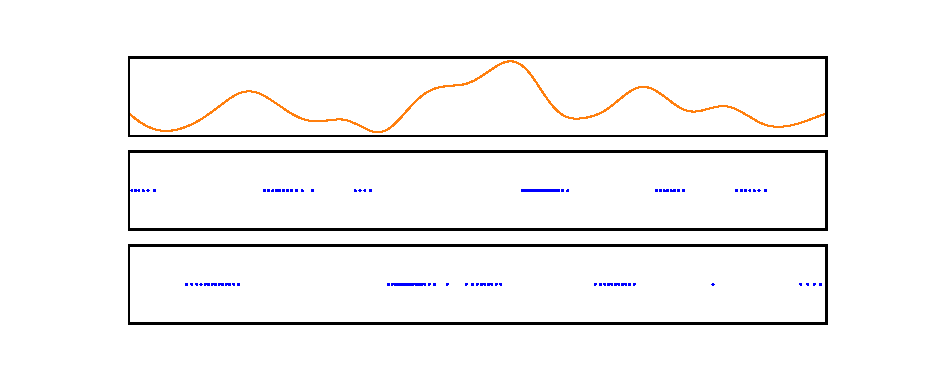
\includegraphics[width = \columnwidth, height=4cm]{figures/delta_modulated_input.eps}
  \caption{The signal (top) is split into two channels, representing the (upward) downward
  magnitude of the signal in the number of spikes.}
  \label{fig:delta_modulated_input}
\end{figure}

Going back to the simulation, one can see that the input to the network is 

\begin{equation*}
  \textnormal{Input} = \mathbf{F^T}x
\end{equation*}
where $\mathbf{F}$ is a matrix of size ($N_x$,$N$). By integrating the spikes using

\begin{equation} \label{recon_input}
  \hat{x}_t = (1-\lambda)\hat{x}_{t-1} + \nu(o^{up}_t - o^{down}_t)
\end{equation}
one can reconstruct a discretized version of the original signal $\hat{x}$ using appropriate values
for $\lambda$ and $\nu$. Using

\[M = \begin{bmatrix}
  1 & -1 & 0 & 0 \\ 
  0 & 0 & 1 & -1
  \end{bmatrix}
\]

the general form of Equation \ref{recon_input} becomes

\begin{equation*}
  \hat{x}_t = (1-\lambda)\hat{x}_{t-1} + \nu Mo_t
\end{equation*}

In order to match the simulation with the DYNAP-SE, one could simply integrate the spikes and transform
the reconstructed signal to get an approximation of the input using

\begin{equation*}
  \textnormal{Input} = \mathbf{F}^T \hat{x} = \mathbf{F}^T((1-\lambda)\hat{x}_{t-1} + Mo_{t-1})
\end{equation*}

This however does not match the setup on the DYNAP-SE since the input is first transformed using $M$, then
integrated and then again transformed using $F$. Contrary, the synapses on the DYNAP-SE first integrate the
incoming spikes and then transform the integrated value using the weights. We therefore introduce a new variable
$I_t$ that symbolizes the current at time $t$ of the synapses. $I_t$ performs a simple integration of the input:

\begin{equation*}
  I_t = (1-\lambda)I_{t-1} + \nu o_t
\end{equation*}

By expanding the recursive definition for $k$ time steps and assuming that $(1-\lambda)^k$ becomes
negligibly small for some $k$ we get that

\begin{equation*}
  \begin{split}
      F^T \hat{x}_t & = F^T((1-\lambda) \hat{x}_{t-1} + \nu Mo_t) \\
      & = F^T((1-\lambda) \;... \;(1-\lambda)( (1-\lambda) \hat{x}_{t-k} + \nu Mo_{t-k+1}) + \nu Mo_{t-k+2} + ... + \nu Mo_t) \\
      & \approx F^T((1-\lambda)^{k-1} \nu Mo_{t-k+1} + (1-\lambda)^{k-2} \nu Mo_{t-k+2} + ... + (1-\lambda)^{0} \nu Mo_{t}) \\
      & = (1-\lambda)^{k-1} \nu F^TMo_{t-k+1} + (1-\lambda)^{k-2} \nu F^TMo_{t-k+2} + ... + (1-\lambda)^0 \nu F^TMo_t
  \end{split}
  \end{equation*}

is equal to

\begin{equation*}
  \begin{split}
      F^T M I_t & = F^T M ((1-\lambda) I_{t-1} + \nu o_t) \\
      & = F^T M((1-\lambda) ... (1-\lambda)( (1-\lambda) I_{t-k} + \nu o_{t-k+1}) + \nu o_{t-k+2} + ... + \nu o_t) \\
      & \approx F^T M((1-\lambda)^{k-1}\nu o_{t-k+1} + (1-\lambda)^{k-2}\nu o_{t-k+2} + ... + (1-\lambda)^{0}\nu o_{t}) \\
      & = (1-\lambda)^{k-1}\nu F^TMo_{t-k+1} + (1-\lambda)^{k-2}\nu F^TMo_{t-k+2} + ... + (1-\lambda)^0 \nu F^TMo_t
  \end{split}
\end{equation*}

We have shown that having real input transformed using a feed-forward matrix $F$ is approximately the same
as integrating a spike train $o_t$ and transforming it using the new matrix $F^TM$. This
scheme was successfully verified in the simulation. Figure \ref{fig:spiking_vs_continous} compares the reconstruction error over time
between the continous-input network and the spiking-input network.
Since the DYNAP-SE is doing the integration implicitly, we can simply set the feed-forward
connections to a discretized version of $F^TM$ and feed the delta modulated input to the chip. Unfortunately,
input precision is lost due to the discretization limit imposed by the spikes and more severly by the
weight resolution on the DYNAP-SE, which will be covered in another section.

\begin{figure}[!htb]
  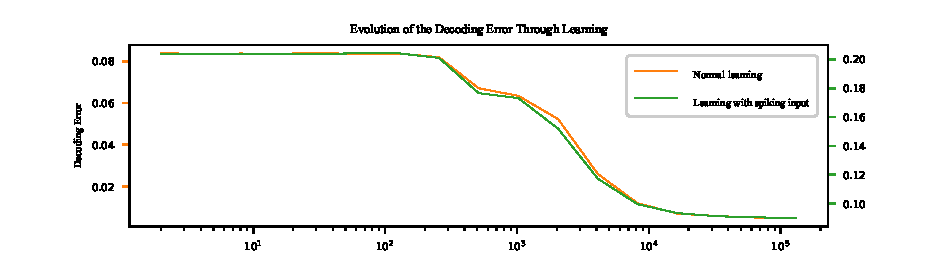
\includegraphics[width = \columnwidth, height=4cm]{figures/error_convergence_use_spiking_vs_normal.eps}
  \caption{While the error convergence of the spiking-input and continous-input network matches,
  the error of the spiking-input network is increased by roughly a factor of 10, due to the
  loss of precision imposed by the spikes (note the green scale).}
  %! Correct caption please
  \label{fig:spiking_vs_continous}
\end{figure}

\newpage

\subsubsection{The weights on-chip} \label{sec:weights}

As pointed out in section \ref{sec:DYNAP-SE}, the fan-in of the DYNAP-SE is relatively small
compared to the fan-out. One neuron can have a maximum of 64 incoming connections.
This becomes a serious problem considering, that in a fully connected network
the number of connections scales quadratically with the number of neurons.
Luckily, the learned matrix exhibits a clear structure, with many values close to zero, so when
discretized, only a few strong inhibitory or excitatory connections remain. Figure \ref{fig:spiking_vs_continous}
compares the continous and discretized weight matrices post learning.

\begin{figure}[!htb]
  \centering
  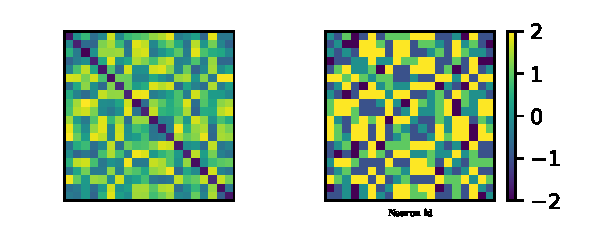
\includegraphics[width =10cm, height=4cm]{figures/weights.pdf}
  \caption{Due to discretization of the matrix, precision is lost. Note that in the right
  plot, only 5 distinct discrete values are visible, while the right matrix is continous.
  However, the global structure is preserved and the matrix is symmetric, as the graph
  should be undirected.}
  \label{fig:spiking_vs_continous}
\end{figure}

In order to understand the process of rescaling the weights, it is important to know that
the DYNAP-SE only has two types of excitatory and inhibitory synapses, respectively.
This means that the weights of these two synapses are actually set pre-learning
and that connections with different weights have to be formed using multiples of these
synapses.
Assuming that we have discrete weights going from $-10$ to $10$, with a resolution of 1, one
can form a connection of strength 3 between two neurons, by forming three seperate connections
using the excitatory synapse. Note that the weights have to be in $\mathbb{Z}$ since
their absolute value indicates the number of synapses used and the sign the type of
synapse ($-$ for inhibition and $+$ for excitation).
Since this is the case, we can simply bin the continous weights and take the indices minus
the number of incoming connections we allow.
To illustrate this consider the following array:
\begin{equation*}
X = [ 0.5 , -0.14,  0.65,  1.52, -0.23, -0.23,  1.58,  0.77, -0.47, 0.54]
\end{equation*}
when binning with $20$ bins (meaning we have $20$ different weights, $-10$ being the smallest and $10$ the biggest),
this yields the following bin edges:
\begin{equation*}
\textnormal{bin edges} = [-0.47, -0.37, -0.26, -0.16, -0.06,  ... \; ,  1.27, 1.37,  1.48,  1.58]
\end{equation*}
Taking the indices of the bins for each value minus the number of the maximum strength per connection (10)
we get the weights:
\begin{equation*}
\textnormal{weights} = [  0,  -6,   1,  10,  -7,  -7,  10,   3, -10,   0]
\end{equation*}

Using this approach causes an undesired effect: Whenever a matrix is rescaled to a certain range,
the information on the weight magnitute, relative to other matrices is lost. A very small matrix at the
beginning of learning compared to a matrix with more extreme weights would have the same magnitude in
the rescaled domain. This undesired effect can be easily resolved by providing a point of reference for the
weight magnitudes in the form of minimum and maximum values in the binning process. These values were obtained
from a previous test run in the simulation. Since it is just a heuristic and learning using the DYNAP-SE produces
different weights, it can happen that weights exceed these limits. In this case they are simply assigned the
minimum or maximum weight. We also verified that using eye-balled values like $-0.5$ and $0.5$ worked. \\

Pushed back by this severe loss in precision and therefore disability to align the off-chip-dynamics with 
on-chip-dynamics, we had to compensate with the right choice of hyperparameters such as the threshold
for the delta modulation and the weights of the inhibitory and excitatory synapses.
To find out the right values, we tried out two different forms of hyperparameter tuning: Simple grid
search and coordinate-descent-inspired grid search. The grid search approach simply iterated through every
possible interleavings of hyperparameters, while the coordinate-descent version picked a parameter to optimize
in each round and remembered the best value for each parameter.
To measure quality of alignment, we passed a random signal through the on- and off-chip network using random
feedforward and recurrent connections and compared the spike trains using different metrics.

%! Try different metrics: von Rossum (already did that), VP, Kreuz

%! Show failed learning when using same weight for inh and exc
%! Later: Show successful learning with crazy activation (but no sparsity)


\subsubsection{Batched updates}

Being a spike-dependent learning rule, weight-updates happen immediately after a spike has been fired.
While being biologically plausible, this type of update is not achievable in our in-the-loop setup.
To match this, we would have to chop up the signal to chunks of size $\Delta T$ and iteratively present,
by $\Delta T$ increasing, parts of the signal and only do an update in the last $\Delta T$, when there 
was a spike. Since a lot of overhead is created when setting the connections on the DYNAP-SE, this becomes
impractical.
Since the future behaviour of the neurons depend on the current weights, it is clear that accumulating the
updates and performing the update at the end of the whole signal is not the same as changing the weights
immediately. Assuming that the signal is relatively small and the recurrent weights do not change too
much during one signal iteration, one can however approximate the online updates with a batch update.
Contrary to the intuitive assumption that we had to scale the accumulated derivatives relative to the
number of updates, we found that learning behaves quite similar to the online setting when the
derivatives are not normalized as can be seen in Figure \ref{fig:batched_update}.

\begin{figure}[!htb]
  \centering
  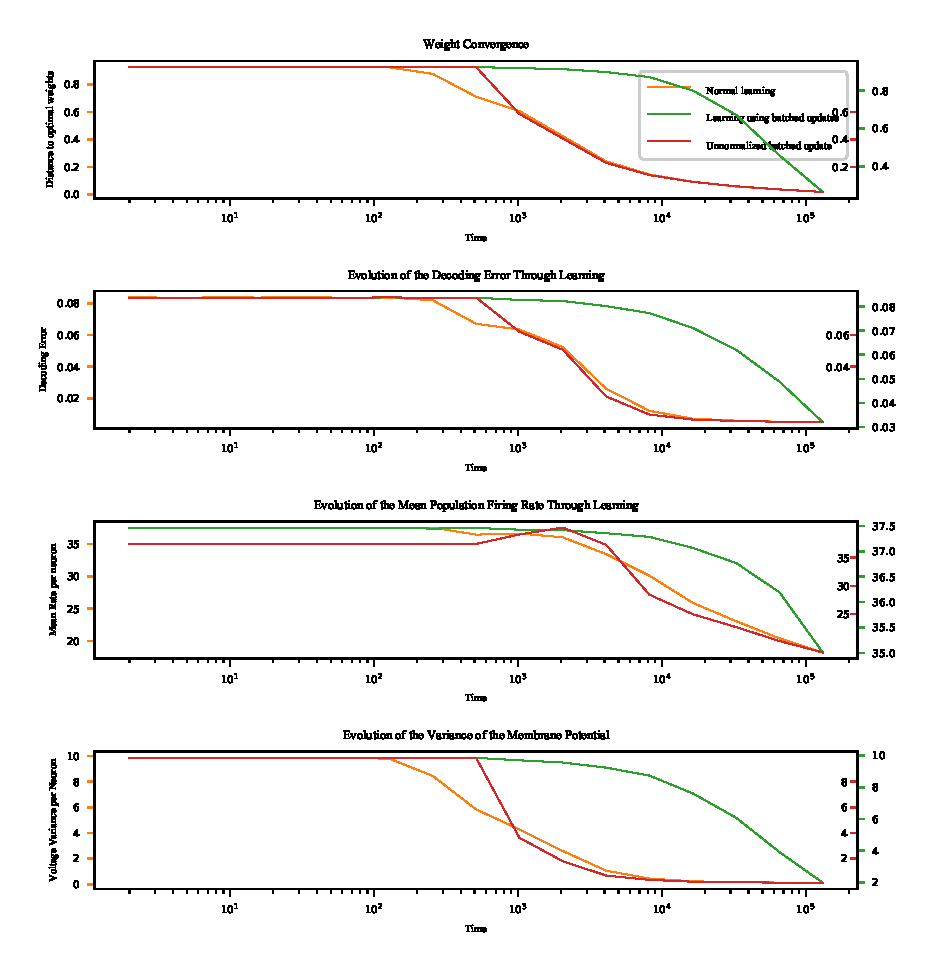
\includegraphics[width = \columnwidth, height=16cm]{figures/convergence_normal_vs_ub_vs_ub_nn.eps}
  \caption{The convergence properties using the batched and online versions of the learning rule. The
  unscaled batched version performs equally well as the online version.}
  \label{fig:batched_update}
\end{figure}

\subsubsection{Further alignment using time-window update}
One fundamental problem that will be resolved in a future chip design, is that
membrane potentials can only be measured using an oscilloscope. This imposes a problem, since
the weight updates rely on the neurons voltages.
To circumvent this limitation, we tried to
reconstruct the voltage $V_{t}$ based on the transformed input $\mathbf{F^T}x(t)$ and the
spikes $o^{DYNAP-SE}(t-1)$. Upon comparison of the reconstructed voltage and the simulation voltage,
we realized that the reconstructed voltage of the population was generally higher than the simulation
version. The reason for this is simple: In the simulation, there can be only one spike per time, but
on the DYNAP-SE, occasionally multiple neurons spiked simultaneously, which we did not take into account.
To resolve this mismatch, we computed the reconstructed voltage using

\begin{equation*}
   V(t) = \mathbf{F^T}x(t) + \mathbf{\Omega}o^{aligned}(t)
\end{equation*}
where $o^{aligned}_k(t)$ is one if $V_k(t-1)$ was the maximum value above threshold
and the DYNAP-SE emitted a spike in a specified time-window $\pm \Delta T$. Note that because
the network dynamics off- and on-chip are not perfectly aligned, we considered a small
time-window, typically of size $\pm 5ms$, instead of checking if there was a spike at exactly
time $t$.
The final pseudo code is illustrated in the following section.

\newpage

\subsubsection{Final pseudo code} \label{sec:pseudo-code}

\IncMargin{1em}
\begin{algorithm}[H]
  \DontPrintSemicolon
  \label{algorithm_chip_in_the_loop}
  \KwIn{Number of training iterations $N_\textnormal{iter}$}
  \KwOut{Learned recurrent matrices $\mathbf{\Omega},\mathbf{\Omega}^{\mathbb{Z}}$}
  \BlankLine
  $\textit{thresh} \leftarrow 0.5$ \;
  $T_{\textnormal{delta modulator up}} \leftarrow 0.05$ \;
  $T_{\textnormal{delta modulator down}} \leftarrow 0.05$ \;
  $\Delta T \leftarrow 5ms$ \;
  $\Omega_{\textnormal{min}} \leftarrow -0.5$ \;
  $\Omega_{\textnormal{max}} \leftarrow 0.5$ \;
  $\mathbf{F} \leftarrow \textnormal{normalize}(\frac{1}{2}\mathcal{N}(\mathbf{0},\mathbf{I}))$ \;
  $\mathbf{F^TM^\mathbb{Z}} \leftarrow \textnormal{discretize}(\mathbf{F^TM})$ \;
  $\textnormal{dynaps.set\_feedforward}(\mathbf{F^TM^\mathbb{Z}})$ \;
  \For{$i \leftarrow 0$ \KwTo $\textnormal{N}_{\textnormal{iter}}$}{
    $\textnormal{Input} \leftarrow \mathcal{N}(\mathbf{0}, \mathbf{I})$ \;
    $\textnormal{Input} \leftarrow A \cdot (\textnormal{Input} \ast w)$ \;

    \For{$t \leftarrow 1$ \KwTo $T_{\textnormal{signal}}$}{
    $X_t \leftarrow (1-\lambda dt)\cdot X_{t-1} + dt \cdot \textnormal{Input}_t$ \;
    }

    $\textnormal{fpga.load\_signal}(X_t)$ \;
    $\mathbf{\Omega}_t \leftarrow \mathbf{\Omega}_{t-1} - \Delta \mathbf{\Omega}$ \;
    $\mathbf{\Omega}_t^{\mathbb{Z}} \leftarrow \textnormal{discretize}(\mathbf{\Omega}_t, \Omega_{\textnormal{min}},\Omega_{\textnormal{max}})$ \;
    $\textnormal{dynaps.set\_recurrent\_connections}(\mathbf{\Omega}_t^{\mathbb{Z}})$ \;
    $\mathbf{O}^{DYNAP-SE} \leftarrow \textnormal{dynaps.run}()$ \;

    \For{$t \leftarrow 1$ \KwTo $T_{\textnormal{signal}}$}{
      $V_t \leftarrow (1-\lambda dt)\cdot V_{t-1} + dt\cdot \mathbf{F^T}\textnormal{Input}_t+\mathbf{\Omega} o^{\textnormal{aligned}}_{t-1}+\epsilon\mathcal{N}(0,1) $ \;
      $(\textnormal{max},k) \leftarrow \textnormal{arg max}(V_t - \textit{thresh}-0.01 \cdot \mathcal{N}(0,1))$ \;
      \eIf{$\textnormal{max} \geq 0 \land \textnormal{has\_spike}(\mathbf{O}^{\textnormal{DYNAP-SE}}_{k,\pm \Delta T})$ }{
          $\Delta \Omega_k \leftarrow \Delta \Omega_k + \epsilon_\Omega \cdot (\beta \cdot (V_t + \mu \cdot r_{t-1}) + \Omega_k + \mu \cdot \mathbf{I})$ \;
          $o_t^{aligned} \leftarrow I_k$ \;
          $r_t \leftarrow r_{t-1} + I_k$ \;
      } {
        $o_t^{aligned} \leftarrow \mathbf{0}$ \;
        $r_t \leftarrow r_{t-1}$ \;
      }
      $r_t \leftarrow (1 - \lambda dt) \cdot r_t$ \;
    }
  }
  \caption{The final pseudo code illustrating the changes made, compared to algorithm
  \ref{algorithm_simulation}. Note for example the batched updates or the discretized feed-forward
  matrix in the beginning. All hyperparameters used can be found in the Appendix. }
\end{algorithm}
\DecMargin{1em}
\vspace{1cm}

\subsection{Results}

Algorithm \ref{algorithm_chip_in_the_loop} was run for $\textnormal{N}_{\textnormal{iter}} = 270$ iterations
with $N = 20$ neurons and $\textnormal{N}_\textnormal{x} = 2$ input signals.
These signals were converted to $\textnormal{N}_{\textnormal{in}} = 4$ channels, representing the
spiking input. In the following figures, $\Delta T = \pm 10 \textnormal{ms}$ was used as a time-window.
To recapitulate, this time-window is used to check, whether the DYNAP-SE emitted a spike in order
to do the update of the neuron with the highest voltage above threshold. We assume that due to
the mismatch, but the general alignment of the DYNAP-SE and the simulation, the neuron with
the highest voltage above threshold in the simulation at time $t$ must have
spiked within a certain $\Delta T$ on the DYNAP-SE.
It should be noted that this scheme can be fooled by simply setting the recurrent weights on-chip
to zero and activating all the neurons, all the time. This way the condition that a spike occurred
within a given time-window is always satisfied and algorithm \ref{algorithm_chip_in_the_loop}
simply becomes a version of the simulation. However, this would render the results useless, as
the spike train does not sparsify and thus does not produce an (almost) optimal code. \\


\begin{figure}[!htb]
  \centering
  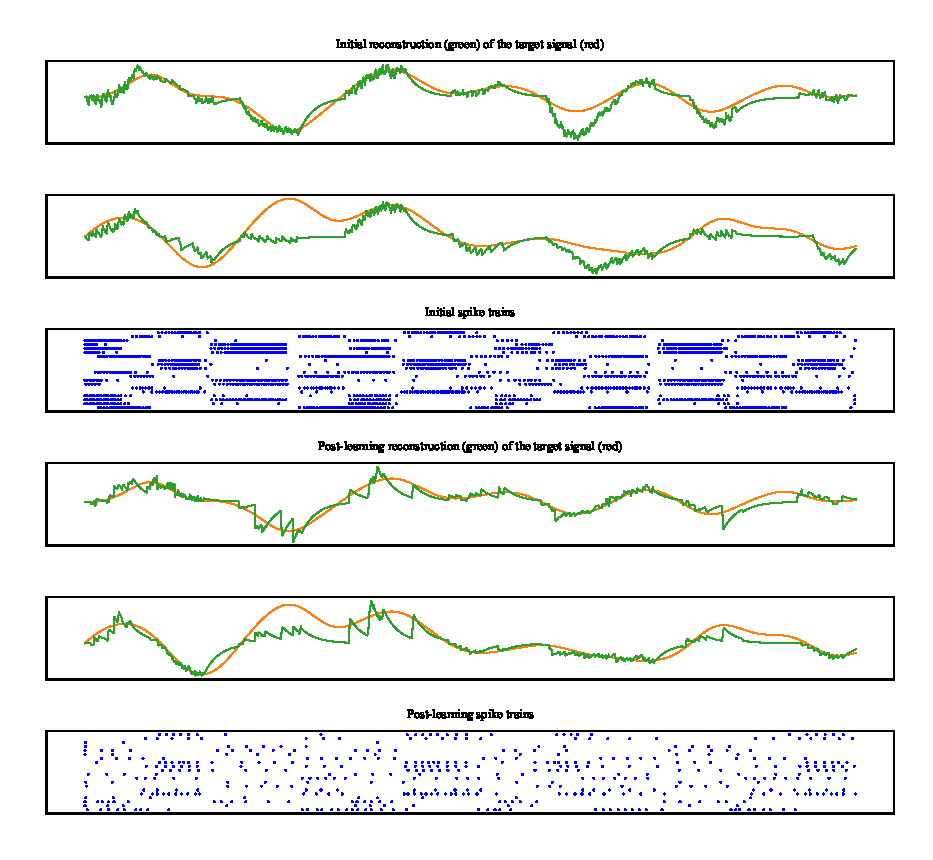
\includegraphics[width = \columnwidth, height=10cm]{figures/DYNAPS_reconstruction.eps}
  \caption{While reducing the reconstruction error, the spike train sparsifies.
  In fact, for this experiment 880 spikes were saved over a period of 1 second, which is more
  than 3 million in one hour. A neuron on the DYNAP-SE consumes roughly 1.68$nJ$, so
  5.04$mJ$ were saved for only 20 neurons.}
  \label{fig:DYNAPS_reconstruction}
\end{figure}

When comparing Figure \ref{fig:DYNAPS_reconstruction} with Figure \ref{fig:reconstruction},
especially the scale of the reconstruction error, it
becomes clear that a lot of precision is lost, due to the simulation-DYNAP-SE mismatch.
Nevertheless, the results show that this setup successfully learns the optimal recurrent matrix,
reduces the mean firing rate, reduces the decoding error and balances the network
(see Figure \ref{fig:DYNAPS_convergence} for convergence behaviour).

\begin{figure}[!htb]
  \centering
  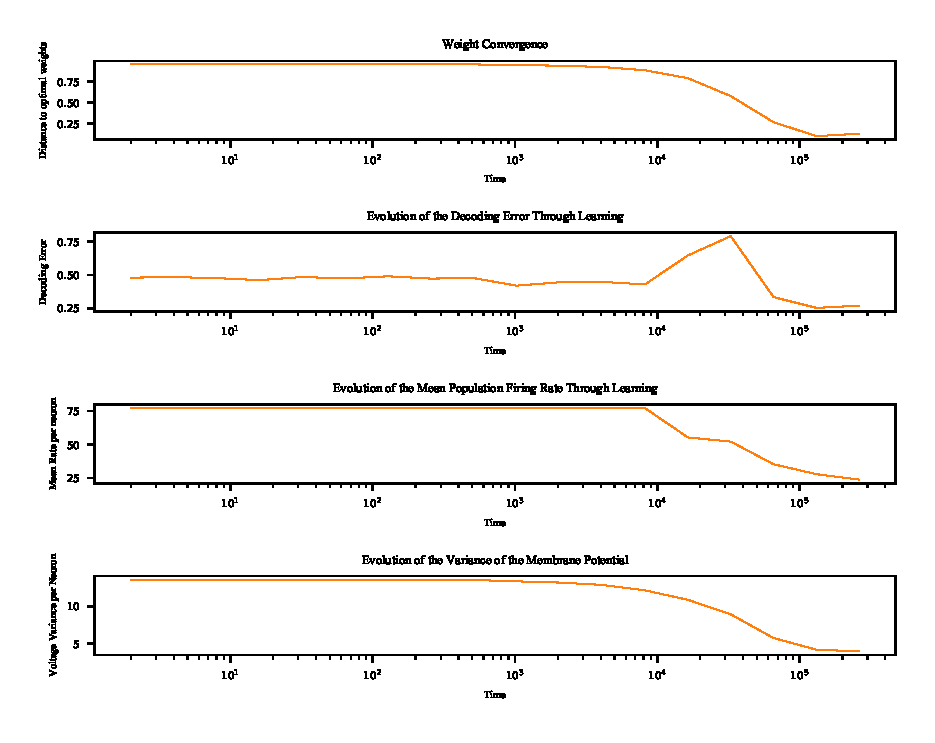
\includegraphics[width = \columnwidth, height=10cm]{figures/DYNAPS_convergence.eps}
  \caption{Besides the decoding error, all variables show stable convergence. Despite the fact that
  overall decoding error is reduced, learning is still unstable and has to be improved using
  an adaptive learning rate (see section \ref{sec:rl}).}
  \label{fig:DYNAPS_convergence}
\end{figure}

\newpage

\subsection{Reinforcement Learning based step size adaptation} \label{sec:rl}
When neural agents interact with their environment, the quality of the internal signal representation
is crucial: Imprecise representations might lead to unsuccessful execution of tasks, which can
potentially cause harm. It is therefore desirable to adapt the learning mechanism to incorporate
abstract rewards, besides the actual learning rules. This is particulary helpful in scenarios where
learning is unstable and a reward can help to adapt the step size taken into the direction of the
negative gradient. To concretise this idea in the context of Reinforcement Learning (\textbf{RL}), the
reward would be the negative reconstruction error and the action would be the appropriate rescaling of the
learning rate. Recently, \cite{xu2019learning} proposed a \textbf{RL}-based approach for learning a
learning-rate schedule. In this work, the reward is a feature comprising many performance indicators
such as validation loss and loss-variance. Reward based adaptation is biologically plausible
and allows to use multiple features,
enabling the construction of more abstract rewards. To avoid hasty corrections based
on short-sighted rewards, we employed a time horizon, which geometrically weighs $n$ rewards from the past
(\cite{Sutton1988}).
We define the reward to be

\begin{equation*} \label{eq:reward}
    r(t) = \frac{\sum_{i=0}^{n}{\theta_{t-i} \cdot \lambda^{-i}}}{\sum_{i=0}^{n}{\lambda^{-i}}}
\end{equation*}

where $\lambda_i$ is the individual reward at time $i$ and $\lambda$ was set to 1.
After a "burn-in" phase, the initial reward is calculated and taken to be the baseline. Subsequent
rewards are then rescaled w.r.t. the inital reward. Depending on how unstable the convergence is,
this reward can be further rescaled by some exponent $\beta$, yielding extremely small step sizes.
The complete update of the learning rate thus becomes:

\begin{equation*}
  \alpha_{t} =
    \begin{cases}
      \alpha_{\textnormal{initial}} \cdot \frac{r(t)}{r(n)} & \text{if $\frac{r(t)}{r(n)} \geq 1$}\\
      \alpha_{\textnormal{initial}} \cdot (\frac{r(t)}{r(n)})^{\beta} & \text{else}
    \end{cases}
\end{equation*}

The effect of this adaptation scheme is made visible in Figure \ref{fig:rewards}, comparing
rewards over time between no adaptation and the reinforcement learning based adaptation in a
noisy learning environment.

\begin{figure}[!htb]
  \centering
  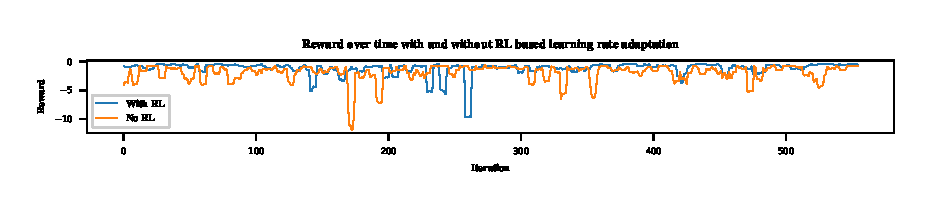
\includegraphics[width = \columnwidth, height=3.0cm]{figures/rl_based_lr_adaptation.eps}
  \caption{When discretizing the weights, convergence becomes unstable, which can be countered
  by an adaptive learning rate. While being biologically plausible, the \textbf{RL} scheme provides
  a flexible learning rate, ensuring more stable convergence. One can see that convergence
  is more stable after approximately 300 iterations.}
  \label{fig:rewards}
\end{figure}

When applying this scheme to the DYNAP-SE setting, learning becomes more stable as Figure \ref{fig:stable}
shows.

\begin{figure}[!htb]
  \centering
  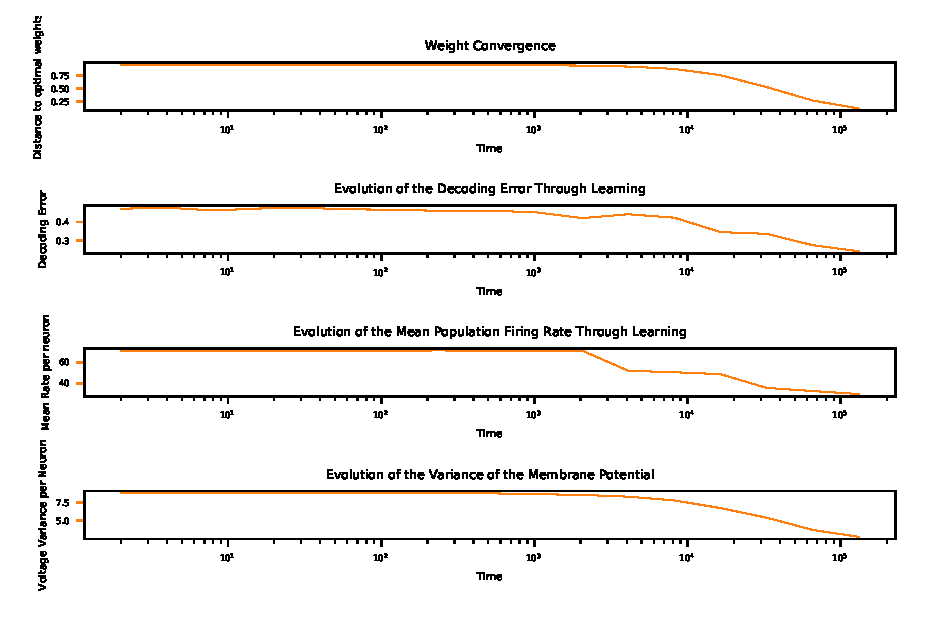
\includegraphics[width = \columnwidth, height=10cm]{figures/DYNAPS_convergence_stable.eps}
  \caption{Convergence using the \textbf{RL}-based scheme becomes more stable (cf. Figure \ref{fig:DYNAPS_convergence}).}
  \label{fig:stable}
\end{figure}

\begin{figure}[!htb]
  \centering
  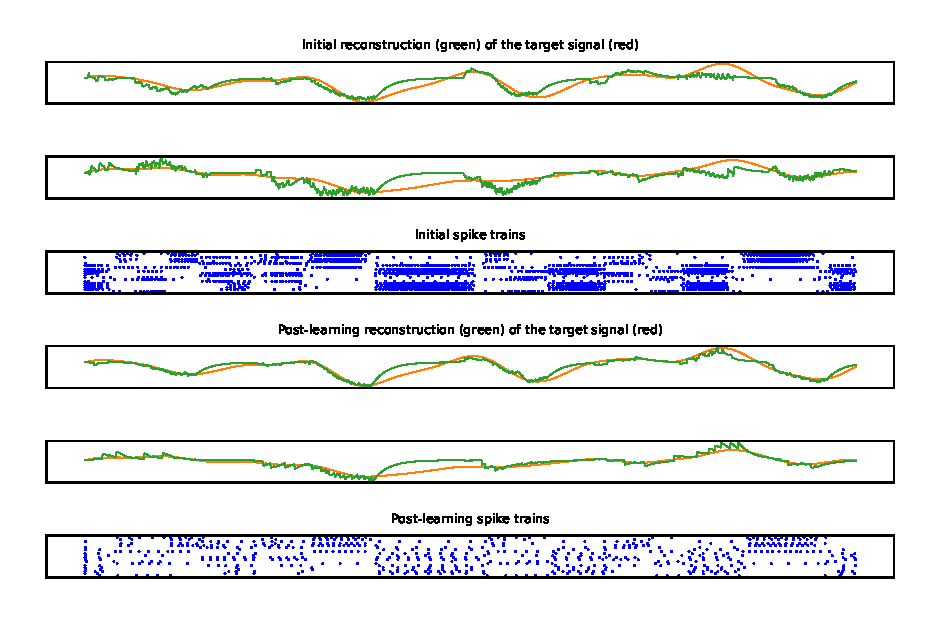
\includegraphics[width = \columnwidth, height=10cm]{figures/DYNAPS_reconstruction_stable.eps}
  \caption{Reconstructed signal using a time-window of $\pm 10ms$ and \textbf{RL}-based lernig rate adaptation with $\beta=10$ and $n=5$.
  Compared to Figure \ref{fig:DYNAPS_reconstruction}, one can see that the reconstruction is indeed more precise.}
  \label{fig:stable_reconstruction}
\end{figure}


\newpage

\section{Discussion}

% Acknowledgements should go at the end, before appendices and references

\acks{I would like to thank my supervisors Sergio Solinas and Giacomo Indiveri for insightful discussions,
showing me valuable papers and teaching me various new concepts.  
I would also like to thank Dimitrii Zendrikov for helpful discussions and joint efforts in fixing bugs
and Christian Machens, who was kind enough to supply me with code
and great insights during my stay at his lab in Lisbon. Finally, I would like to thank my
Co-Supervisor Onur Mutlu for making this thesis possible by supervising it.}

\newpage

\vskip 0.2in
\bibliography{bibliography}

\end{document}